% Options for packages loaded elsewhere
\PassOptionsToPackage{unicode}{hyperref}
\PassOptionsToPackage{hyphens}{url}
%
\documentclass[
  ignorenonframetext,
]{beamer}
\usepackage{pgfpages}
\setbeamertemplate{caption}[numbered]
\setbeamertemplate{caption label separator}{: }
\setbeamercolor{caption name}{fg=normal text.fg}
\beamertemplatenavigationsymbolsempty
% Prevent slide breaks in the middle of a paragraph
\widowpenalties 1 10000
\raggedbottom
\setbeamertemplate{part page}{
  \centering
  \begin{beamercolorbox}[sep=16pt,center]{part title}
    \usebeamerfont{part title}\insertpart\par
  \end{beamercolorbox}
}
\setbeamertemplate{section page}{
  \centering
  \begin{beamercolorbox}[sep=12pt,center]{part title}
    \usebeamerfont{section title}\insertsection\par
  \end{beamercolorbox}
}
\setbeamertemplate{subsection page}{
  \centering
  \begin{beamercolorbox}[sep=8pt,center]{part title}
    \usebeamerfont{subsection title}\insertsubsection\par
  \end{beamercolorbox}
}
\AtBeginPart{
  \frame{\partpage}
}
\AtBeginSection{
  \ifbibliography
  \else
    \frame{\sectionpage}
  \fi
}
\AtBeginSubsection{
  \frame{\subsectionpage}
}
\usepackage{amsmath,amssymb}
\usepackage{iftex}
\ifPDFTeX
  \usepackage[T1]{fontenc}
  \usepackage[utf8]{inputenc}
  \usepackage{textcomp} % provide euro and other symbols
\else % if luatex or xetex
  \usepackage{unicode-math} % this also loads fontspec
  \defaultfontfeatures{Scale=MatchLowercase}
  \defaultfontfeatures[\rmfamily]{Ligatures=TeX,Scale=1}
\fi
\usepackage{lmodern}
\usetheme[]{Madrid}
\ifPDFTeX\else
  % xetex/luatex font selection
\fi
% Use upquote if available, for straight quotes in verbatim environments
\IfFileExists{upquote.sty}{\usepackage{upquote}}{}
\IfFileExists{microtype.sty}{% use microtype if available
  \usepackage[]{microtype}
  \UseMicrotypeSet[protrusion]{basicmath} % disable protrusion for tt fonts
}{}
\makeatletter
\@ifundefined{KOMAClassName}{% if non-KOMA class
  \IfFileExists{parskip.sty}{%
    \usepackage{parskip}
  }{% else
    \setlength{\parindent}{0pt}
    \setlength{\parskip}{6pt plus 2pt minus 1pt}}
}{% if KOMA class
  \KOMAoptions{parskip=half}}
\makeatother
\usepackage{xcolor}
\newif\ifbibliography
\usepackage{graphicx}
\makeatletter
\def\maxwidth{\ifdim\Gin@nat@width>\linewidth\linewidth\else\Gin@nat@width\fi}
\def\maxheight{\ifdim\Gin@nat@height>\textheight\textheight\else\Gin@nat@height\fi}
\makeatother
% Scale images if necessary, so that they will not overflow the page
% margins by default, and it is still possible to overwrite the defaults
% using explicit options in \includegraphics[width, height, ...]{}
\setkeys{Gin}{width=\maxwidth,height=\maxheight,keepaspectratio}
% Set default figure placement to htbp
\makeatletter
\def\fps@figure{htbp}
\makeatother
\setlength{\emergencystretch}{3em} % prevent overfull lines
\providecommand{\tightlist}{%
  \setlength{\itemsep}{0pt}\setlength{\parskip}{0pt}}
\setcounter{secnumdepth}{-\maxdimen} % remove section numbering
\ifLuaTeX
  \usepackage{selnolig}  % disable illegal ligatures
\fi
\usepackage{bookmark}
\IfFileExists{xurl.sty}{\usepackage{xurl}}{} % add URL line breaks if available
\urlstyle{same}
\hypersetup{
  pdftitle={5 - Equalização de canais de comunicação},
  pdfauthor={TDI Course},
  hidelinks,
  pdfcreator={LaTeX via pandoc}}

\title{5 - Equalização de canais de comunicação}
\author{TDI Course}
\date{}

\begin{document}
\frame{\titlepage}

\section{Transmissão Digital da
Informação}\label{transmissuxe3o-digital-da-informauxe7uxe3o}

\section{Equalização em canais de
comunicação}\label{equalizauxe7uxe3o-em-canais-de-comunicauxe7uxe3o}

\begin{frame}{Equalização em canais de comunicação}

\includegraphics{figuras/Fig1.png}

Fig.1: Diagrama de blocos de um sistema de transmissão digital genérico.
\end{frame}

\begin{frame}{Canais distorcivos e limitados em banda}
\phantomsection\label{canais-distorcivos-e-limitados-em-banda}
Na análise que segue, considere que o canal de comunicações pode ser
modelado como um sistema linear com uma resposta ao impulso \(h(t)\) e
resposta em frequência \(H(f)\) limitada a uma banda de \(B\) Hz, de
modo que

\begin{equation}
H(f) = \begin{cases}|H(f)|e^{\theta(f)}, & |f|<B \\ 0, & \text { caso contrário.}\end{cases}
\end{equation}

e \(H(f) = \int_{-\infty}^{\infty}h(t)e^{-2\pi f t} dt\), \(|H(f)|\) é a
resposta de amplitude e \(\theta(f)\) a resposta de fase do canal. A
partir da resposta de fase podemos definir o \emph{atraso de grupo} como

\begin{equation}
\tau(f)=-\frac{1}{2 \pi} \frac{d \theta(f)}{d f}.
\end{equation}

O atraso de grupo corresponde ao intervalo de tempo com que cada
componente de frequência do sinal transmitido atravessa o canal linear.
\end{frame}

\begin{frame}

Um canal linear causará distorção nos sinais por ele transmitidos se
\(|H(f)|\) não for constante ou \(\theta(f)\) não for uma função linear
de \(f\), ou seja, se o atraso de grupo não for constante para todos os
componentes de frequência dentro da banda do canal.

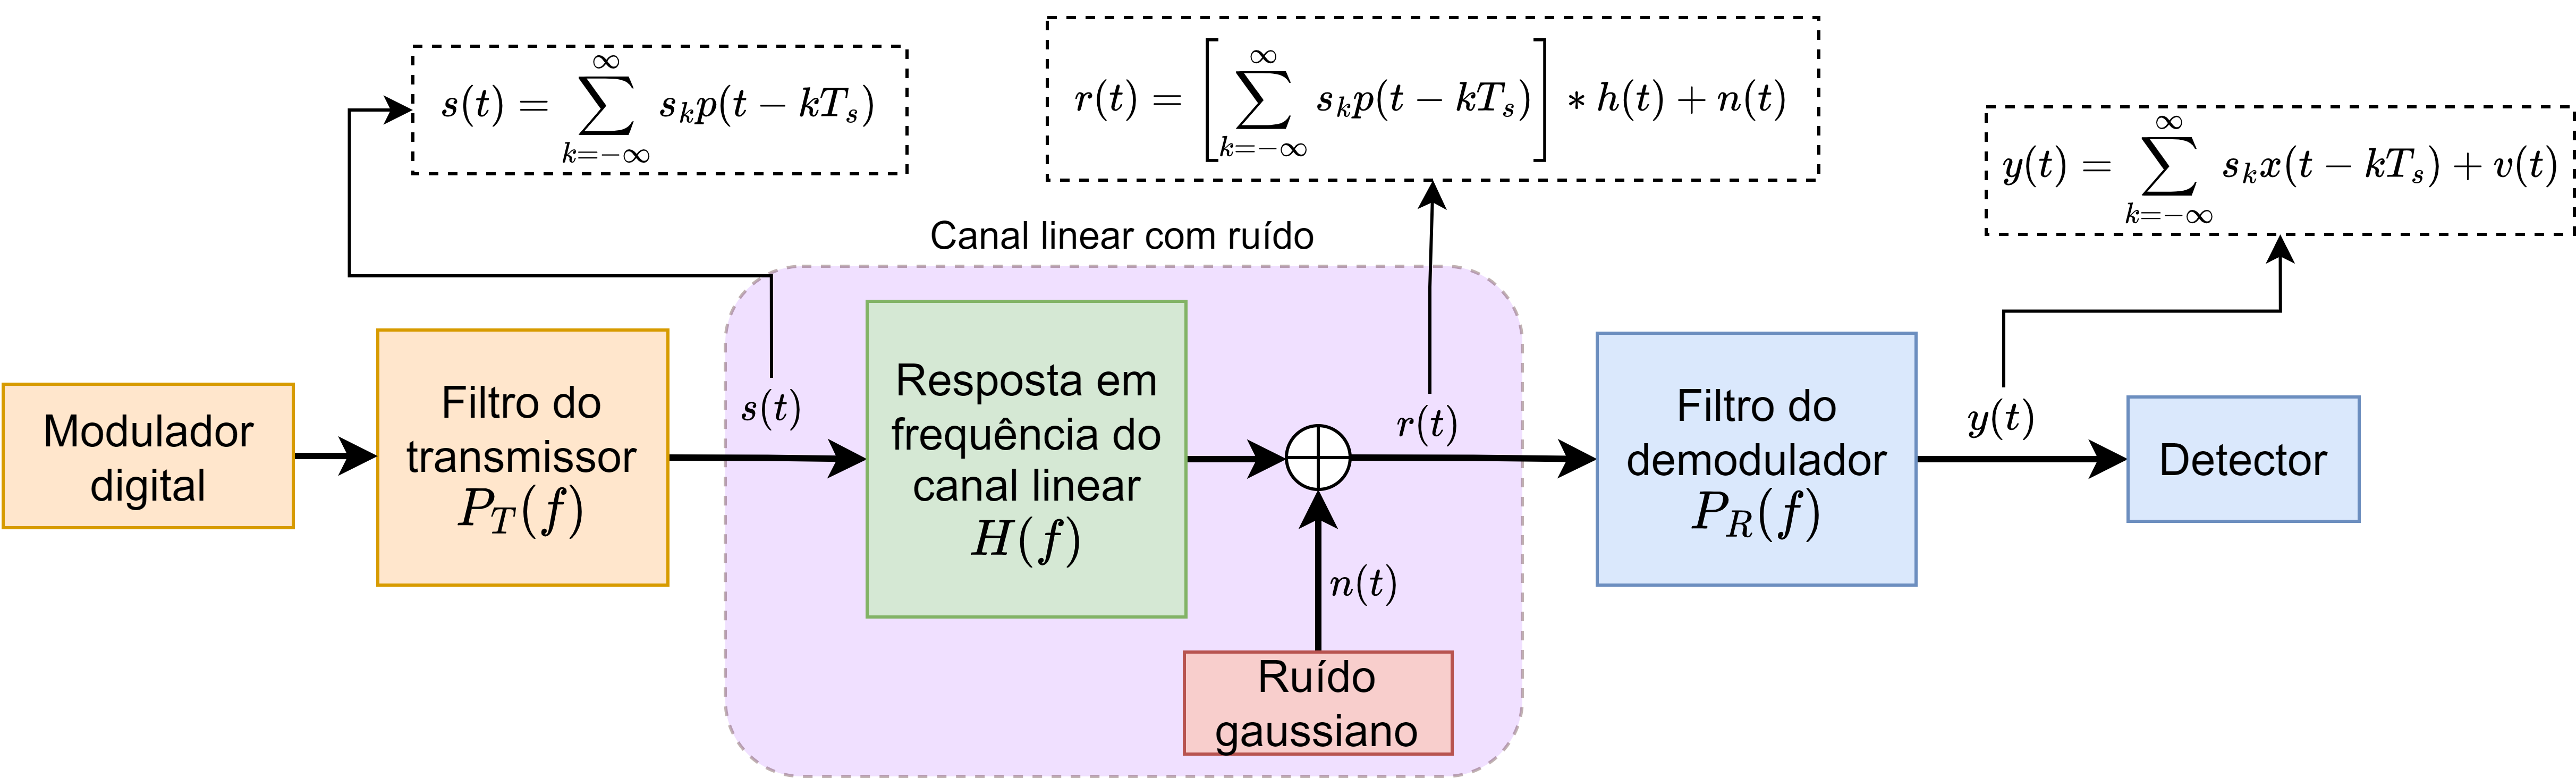
\includegraphics{figuras/Fig14.png}

Fig.2: Esquemático de um sistema de transmissão digital via canal linear
e AWGN.

\end{frame}

\begin{frame}{Interferência intersimbólica (ISI)}
\phantomsection\label{interferuxeancia-intersimbuxf3lica-isi}
Assuma que no receptor o sinal \(r(t)\) é filtrado e amostrado nos
instantes \(t=qT_s + \tau_{0}, q=0, 1, \ldots\). Seja a saída do filtro
do receptor dada por

\begin{equation}
y(t)=\sum_{k=-\infty}^{\infty} s_k x(t-kT_s) + v(t)
\end{equation}

em que o pulso \(x(t)\) é o resultado da convolução do pulso original
\(p(t)\) com a resposta ao impulso do canal \(h(t)\) e a resposta ao
impulso do filtro do recetor \(p_{R}(t)\) e \(v(t)\) é o resultado da
convolução entre o ruído gaussiano na entrada do receptor e
\(p_{R}(t)\). 
\end{frame}

\begin{frame}
Considerando apenas a representação discreta do sinal,
temos \begin{equation}\label{ISI_eq1}
y[k]=s[k] + \sum_{\substack{n=-\infty \\ n \neq k}}^{\infty} s[n] x[k-n] + v[k], \quad k=0,1, \ldots
\end{equation}

Em (\ref{ISI_eq1}), temos que \(s[k]\) é o símbolo transmitido no
intervalo de sinalização \(k\). Já o termo
\(\sum_{\substack{n=-\infty \\ n \neq k}}^{\infty} s[n] x[k-n]\)
representa a interferência causada em \(s[k]\) pelos demais símbolos
transmitidos, denominada \textbf{interferência intersimbólica}
(\emph{intersymbol interference} - ISI). Por fim, \(v[k]\) é uma
variável aleatória representado o ruído no instante de sinalização
\(k\).

\end{frame}
\begin{frame}{Minimização do critério do pico de distorção (\emph{peak
distortion criterion})}
\phantomsection\label{minimizauxe7uxe3o-do-crituxe9rio-do-pico-de-distoruxe7uxe3o-peak-distortion-criterion}
Considere que utilizaremos como equalizador de \(y[k]\) um filtro linear
discreto no tempo com resposta ao impulso \(c[m]\), de modo que \[
z[k]=\sum_{m=-\infty}^{\infty} c[m]\,y[k-m].
\] onde \(z[k]\) é a saída do equalizador.

Substituindo \(y[k]\) e reorganizando, temos \[
z[k]=\sum_{n=-\infty}^{\infty} s[n]\,g[k-n] + w[k],
\] onde a resposta equivalente é \[
g[\ell]\triangleq c[\ell]\ast x[\ell] = \sum_{m=-\infty}^{\infty} c[m]\,x[\ell-m],
\qquad
w[k]\triangleq \sum_{m=-\infty}^{\infty} c[m]\,v[k-m].
\] 
\end{frame}

\begin{frame}
Assim, \[
z[k]=s[k]g[0]+\sum_{\substack{n=-\infty \\ n \neq k}}^{\infty} s[n]g[k-n]+w[k].
\]

Normalizando o resultado por \(g[0]\), temos

\[
z[k]=s[k]+\sum_{\substack{n=-\infty \\ n \neq k}}^{\infty} s[n]g[k-n]+w[k].
\]

Defina a distorção de pico como a energia dos termos fora do pico
desejado (assumindo pico em \(\ell=0\)): \[
D(c) \triangleq \sum_{\substack{\ell=-\infty \\ \ell \neq 0}}^{\infty} |g[\ell]|^2.
\]

\end{frame}

\begin{frame}
Como \(D(c)\ge 0\), o mínimo global ocorre quando \(D(c)=0\), isto é,

\[
g[\ell] = \delta[\ell] =
\begin{cases}
1, & \ell = 0 \\
0, & \ell \neq 0
\end{cases}
\]

Como \(g[\ell]=c[\ell]\ast x[\ell]\), a condição ótima é \[
c[\ell]\ast x[\ell]=\delta[\ell].
\]

No domínio-\(z\), \[
C(z)X(z) = 1,
\qquad
C(z)=\frac{1}{X(z)}.
\]

Sabemos que \(X(z)=P_T(z)H(z)P_R(z)\). Logo, se \(P_T(z)\) e \(P_R(z)\)
resultarem num pulso livre de ISI, basta que \[C(z)=\frac{1}{H(z)},\]

para que a saída do equalizador esteja livre de ISI. Este equalizador é
conhecido como equalizador de zero-forçado (\emph{zero-forcing}- ZF
equalizer) .

\end{frame}

\begin{frame}
Para garantir que o equalizador ZF seja \textbf{estável}, escolhe o
canal deve ter uma função de transferência de \textbf{fase mínima}, isto
é, com todos os zeros dentro do círculo unitário.

Considere que o canal \(H(z)\) pode ser representado pela função de
transferência \[
H(z)=\prod_{i=1}^{N}\left(1-a_i z^{-1}\right),
\] com zeros em \(z=a_i\). Assim, \(H(z)\) será de fase-mínima se
\(|a_i|<1\) para todo \(i\).
\end{frame}

\begin{frame}{Exemplo: aplicação de um equalizador ZF para compensação
de ISI num canal linear}
\phantomsection\label{exemplo-aplicauxe7uxe3o-de-um-equalizador-zf-para-compensauxe7uxe3o-de-isi-num-canal-linear}
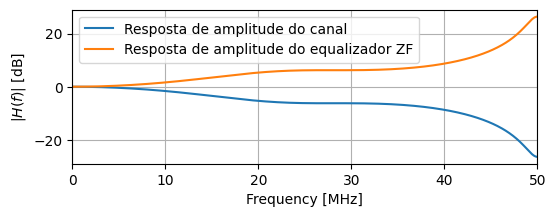
\includegraphics{figuras/nb4_out_0.png}
\end{frame}

\begin{frame}
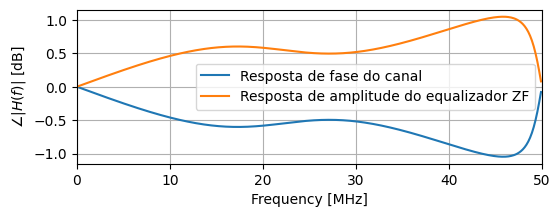
\includegraphics{figuras/nb4_out_1.png}
\end{frame}

\begin{frame}
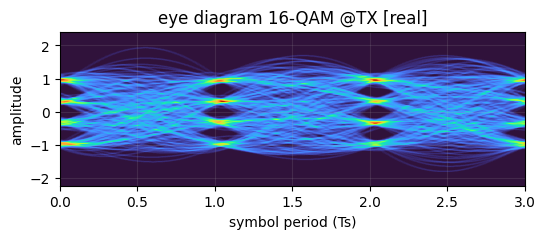
\includegraphics{figuras/nb4_out_2.png}

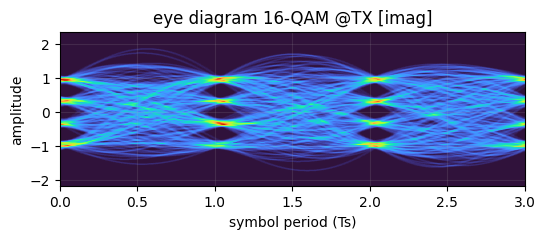
\includegraphics{figuras/nb4_out_3.png}
\end{frame}

\begin{frame}
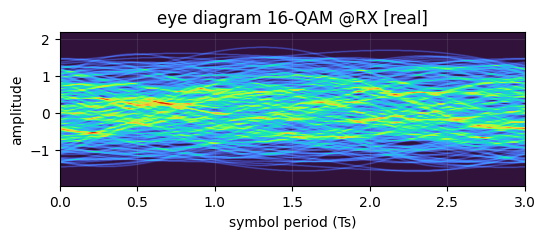
\includegraphics{figuras/nb4_out_4.png}

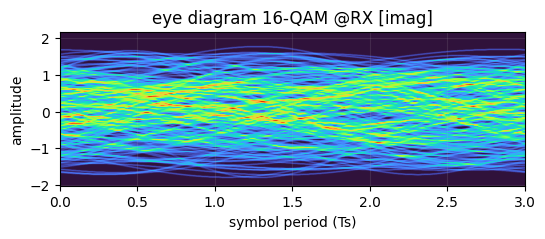
\includegraphics{figuras/nb4_out_5.png}
\end{frame}

\begin{frame}
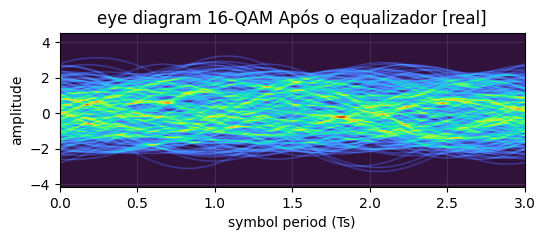
\includegraphics{figuras/nb4_out_6.png}

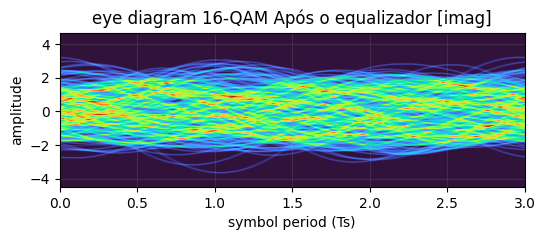
\includegraphics{figuras/nb4_out_7.png}
\end{frame}

\begin{frame}
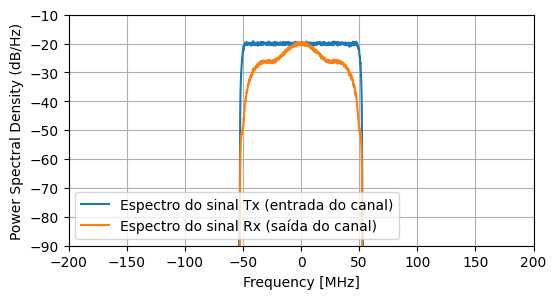
\includegraphics{figuras/nb4_out_8.png}

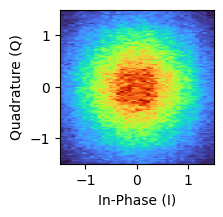
\includegraphics{figuras/nb4_out_9.png}
\end{frame}

\begin{frame}
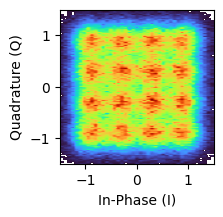
\includegraphics{figuras/nb4_out_10.png}

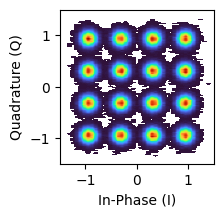
\includegraphics{figuras/nb4_out_11.png}
\end{frame}

\begin{frame}{Minimização do critério de erro médio quadrático
(\textbf{\emph{mean-squared-error}} - \textbf{MSE})}
\phantomsection\label{minimizauxe7uxe3o-do-crituxe9rio-de-erro-muxe9dio-quadruxe1tico-mean-squared-error---mse}
A utilização do critério do pico de distorção não leva em conta o ruído
aditivo que afeta o sinal. Por esta razão, caso a resposta em frequência
do canal atenue fortemente algum componente de frequência dentro da
banda do sinal, o equalizador ZF aplicará um ganho correspondente para
restaurar a potência de sinal. Entretanto, o mesmo ganho será aplicado
ao ruído, o que pode reduzir severamente a \(\mathrm{SNR}\) na entrada
do detector, reduzindo o desempenho da transmissão.

Desse modo, o uso de equalizadores ZF é mais apropriado em situações
onde a resposta em frequência do canal é relativamente plana, ou a
\(\mathrm{SNR}\) do sistema é elevada. Quando essas condições não são
atendidas, uma melhor alternativa seria otimizar os coeficientes do
filtro equalizador com relação a um critétio que leve em conta tanto o
efeito da ISI como do ruído, de modo a obter o melhor compromisso em
termos de equalização e desempenho. 
\end{frame}

\begin{frame}
Um critério que atende esse cenário
é o erro médio quadrático (\textbf{\emph{mean-squared error}} -
\textbf{MSE}) entre o sinal na entrada do canal e a saída do
equalizador. O conjunto de coeficientes que minimiza o MSE é conhecido
como solução MMSE ou equalizador MMSE.
\end{frame}
\begin{frame}{Determinação do equalizador MMSE}
\phantomsection\label{determinauxe7uxe3o-do-equalizador-mmse}
Assuma que saída do filtro casado no receptor pode ser expressa como

\[
y[k]=\sum_{n=0}^{N-1} h[n]s[k-n]+\eta[k]
\]

em que \(\eta[k] \sim \mathcal{N}(0,\sigma_\eta^2)\) e
\(R_{\eta\eta}[m] = \mathbb{E}\{\eta[k]\eta^*[k-m]\}=\sigma_n^2\delta[m]\)

Considerando que um equalizador com \(N_1\) precursores e \(N_2\)
pós-cursores, o comprimento total do filtro será $L=N_1+N_2+1$
\[
\mathbf{y}[k]=[y[k-N_1],\ldots, y[k], \ldots ,y[k+N_2]]^T,
\]
\[
\mathbf{c}=[c[-N_1],\ldots, c[0], \ldots ,c[N_2]]^T,
\]
\[ \mathbf{s}[k] = \left[s[k-N_1], s[k-N_1+1],\ldots,s[k],\ldots, s[k+N_2+N]\right]^T\]
\[
\mathbf{\eta}[k]=[\eta[k-N_1],\ldots, \eta[k], \ldots ,\eta[k+N_2]]^T,
\]
\end{frame}

\begin{frame}
O mesmo modelo pode ser escrito como uma matriz Toeplitz

\[
\mathbf{y}[k]=\mathbf{H}\mathbf{s}[k]+\mathbf{\eta}[k],
\]

onde estrutura de \(\mathbf{H}\) é da forma

\[
\mathbf{H}=
\begin{bmatrix}
h[0] & h[1]  & \cdots & h[N-1] & 0 & \cdots & 0\\
0 & h[0] & h[1]  & \cdots & h[N-1] & \ddots & \vdots\\
\vdots & \ddots & \ddots & \ddots & \ddots & \ddots & 0\\
0 & \cdots & 0 & h[0] & h[1]  & \cdots & h[N-1]
\end{bmatrix}.
\]

\[
\mathbf{H}\in\mathbb{C}^{L\times L_x},
\qquad
L=N_1+N_2+1,
\qquad
L_x=N_1+N_2+N.
\]

\end{frame}

\begin{frame}
Seja a saída do equalizador no instante \(k\) dada por \[
\hat s[k]=\mathbf{c}^H\mathbf{y}[k].
\]

temos que o erro entre a saída do filtro e a sequência de símbolos
transmitida é dada por
\(e[k]\triangleq s[k]-\mathbf{c}^H\mathbf{y}[k]\).

Deseja-se obter o vetor de coeficientes \(\mathbf{c}\) que minimiza a
função objetivo definida como o valor esperado do erro-médio quadrático

\[
J(\mathbf{c})\triangleq \mathbb{E}\{|e[k]|^2\} = \mathbb{E}\{e[k]e^*[k]\}.
\]

\end{frame}

\begin{frame}
Expandindo a funcão custo: \[
\begin{aligned}
J(\mathbf{c})
 & =
\mathbb{E}\left\{
\left(s[k]-\mathbf{c}^H\mathbf{y}[k]\right)
\left(s^*[k]-\mathbf{y}^H[k]\mathbf{c}\right)
\right\}\\
&=\mathbb{E}\{|s[k]|^2\}
-
\mathbb{E}\{s[k]\mathbf{y}^H[k]\}\mathbf{c}
-
\mathbf{c}^H\mathbb{E}\{\mathbf{y}[k]s^*[k]\}
+
\mathbf{c}^H\mathbb{E}\{\mathbf{y}[k]\mathbf{y}^H[k]\}\mathbf{c}.
\end{aligned}
\]

Como \(\mathbf{c}^H\mathbf{y}[k]\) é um escalar complexo, temos
\(\mathbf{c}^H\mathbf{y}[k] = (\mathbf{y}^H[k]\mathbf{c})^*\), e assim

\[
J(\mathbf{c})
=
\mathbb{E}\{|s[k]|^2\}
-
(\mathbf{c}^H\mathbb{E}\{\mathbf{y}[k]s^*[k]\})^*
-
\mathbf{c}^H\mathbb{E}\{\mathbf{y}[k]s^*[k]\}
+
\mathbf{c}^H\mathbb{E}\{\mathbf{y}[k]\mathbf{y}^H[k]\}\mathbf{c}.
\]

Definimos a matriz de correlação do vetor de entrada do filtro
equalizador \(\mathbf{R}_{yy}\) como
\[
\mathbf{R}_{yy}\triangleq \mathbb{E}\{\mathbf{y}[k]\mathbf{y}^H[k]\}\in\mathbb{C}^{L\times L}
\]
o vetor de correlação cruzada entre entrada e saída do equalizador
\(\mathbf{p}_{ys}\) como \[
\mathbf{p}_{ys}\triangleq \mathbb{E}\{\mathbf{y}[k]s^*[k]\}\in\mathbb{C}^{L}.
\]
e a variância da sequência de símbolos \(\sigma_s^2\) como \[
\sigma_s^2 \triangleq \mathbb{E}\{|s[k]|^2\}
\]

\end{frame}

\begin{frame}
e teremos

\[
\begin{aligned}
J(\mathbf{c})
& =
\sigma_s^2
-
(\mathbf{c}^H\mathbf{p}_{ys})^*
-
\mathbf{c}^H\mathbf{p}_{ys}
+
\mathbf{c}^H\mathbf{R}_{yy}\mathbf{c}.
\\
& =
\sigma_s^2
-
\mathbf{p}_{ys}^H\mathbf{c}
-
\mathbf{c}^H\mathbf{p}_{ys}
+
\mathbf{c}^H\mathbf{R}_{yy}\mathbf{c}.
\end{aligned}
\]

Derivar \(J(\mathbf{c})\) com relação a \(\mathbf{c}^*\) no cálculo de
Wirtinger equivale a derivar \(J(\mathbf{c}_R, \mathbf{c}_I)\) com
relação a \(\mathbf{c}_R\) e \(\mathbf{c}_I\) no cálculo real.

Assim, encontrar o mínimo de \(J(\mathbf{c})\) implica calcular o vetor
de coeficientes \(\mathbf{c}\) de tal forma que o gradiente de
\(J(\mathbf{c})\) seja nulo. No cálculo de Wirtinger, isso significa
\[\frac{\partial J(\mathbf{c})}{\partial \mathbf{c^*}}=0.\]
Utilizando os resultados do cálculo de Wirtinger \[
\frac{\partial}{\partial \mathbf{c}^*}(\mathbf{c}^H\mathbf{R}_{yy}\mathbf{c})=\mathbf{R}_{yy}\mathbf{c},
\qquad
\frac{\partial}{\partial \mathbf{c}^*}(\mathbf{c}^H\mathbf{p}_{ys})=\mathbf{p}_{ys},
\qquad
\frac{\partial}{\partial \mathbf{c}^*}(\mathbf{p}_{ys}^H\mathbf{c})=0.
\]
obtemos as equações de Wiener-Hopf cuja solução
\[
\mathbf{R}_{yy}\mathbf{c}_{\text{MMSE}}=\mathbf{p}_{ys}
\quad\Longrightarrow\quad
\boxed{\mathbf{c}_{\text{MMSE}}=\mathbf{R}_{yy}^{-1}\mathbf{p}_{ys}}.
\]
\end{frame}

\begin{frame}
\[
\mathbf{R}_{yy}
=\mathbb{E}\{\mathbf{y}[k]\mathbf{y}[k]^H\}
=\mathbf{H}\mathbf{R}_{ss}\mathbf{H}^H+\mathbf{R}_{\eta\eta}.
\]
\[
\mathbf{R}_{\eta\eta} \triangleq \mathbb{E}\left\{\mathbf{\eta}[k] \mathbf{\eta}[k]^H\right\}\quad\Longrightarrow\quad
\mathbf{R}_{\eta\eta}=\sigma_\eta^2\mathbf{I}_L.
\]

Caso a sequência de símbolos seja estacionária e descorrelacionada, ou
seja \(R_{ss}[m]=\sigma_s^2\delta[m]\), temos:
\(\mathbf{R}_{ss} = \sigma_s^2 \mathbf{I}_{L_x}\)
\[
\boxed{\mathbf{R}_{yy}=\sigma_s^2\mathbf{H}\mathbf{H}^H+\sigma_\eta^2\mathbf{I}_L.}
\]
Correlação cruzada \[
\mathbf{p}_{yx}=\mathbb{E}\{\mathbf{y}[k]s^*[k]\}
=\mathbf{H}\,\mathbb{E}\{\mathbf{s}[k]s^*[k]\}
\triangleq \mathbf{H}\sigma_s^2 \mathbf{e}_{N_1}.
\]
\[
\boxed{\mathbf{p}_{ys}=\sigma_s^2\mathbf{H}\mathbf{e}_{N_1}.}
\]
\[
\mathbf{c}_{\text{MMSE}}
=
\big(\sigma_s^2\mathbf{H}\mathbf{H}^H+\sigma_\eta^2\mathbf{I}_L\big)^{-1}
\big(\sigma_s^2\mathbf{H}\mathbf{e}_{N_1}\big).
\]
\end{frame}

\begin{frame}
e seja \(\mathrm{SNR}=\sigma_s^2/\sigma_\eta^2\), temos

\[
\boxed{
\mathbf{c}_{\text{MMSE}}
=
\left(\mathbf{H}\mathbf{H}^H+\frac{1}{\mathrm{SNR}}\mathbf{I}_L\right)^{-1}
\left(\mathbf{H}\mathbf{e}_{N_1}\right).
}
\]
\end{frame}

\begin{frame}{Exemplo: aplicação de um equalizador MMSE para compensação
de ISI num canal linear}
\phantomsection\label{exemplo-aplicauxe7uxe3o-de-um-equalizador-mmse-para-compensauxe7uxe3o-de-isi-num-canal-linear}
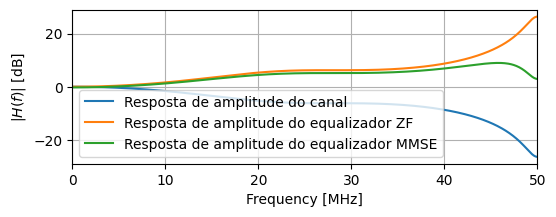
\includegraphics{figuras/nb4_out_12.png}
\end{frame}

\begin{frame}
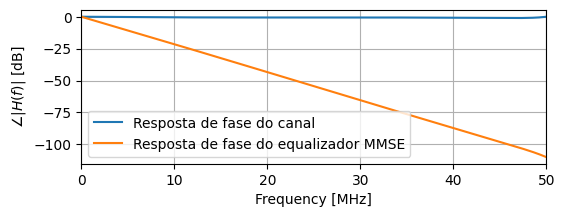
\includegraphics{figuras/nb4_out_13.png}
\end{frame}

\begin{frame}
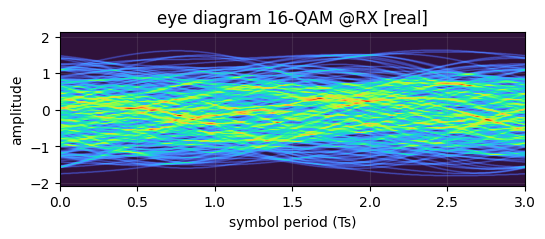
\includegraphics{figuras/nb4_out_14.png}
\end{frame}

\begin{frame}
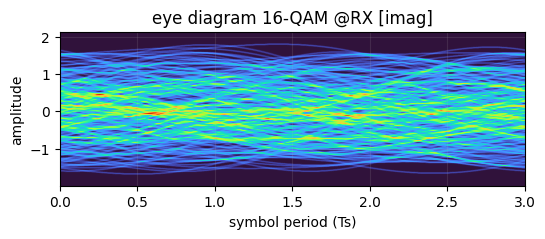
\includegraphics{figuras/nb4_out_15.png}
\end{frame}

\begin{frame}
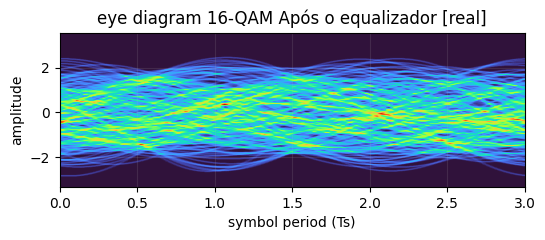
\includegraphics{figuras/nb4_out_16.png}
\end{frame}

\begin{frame}
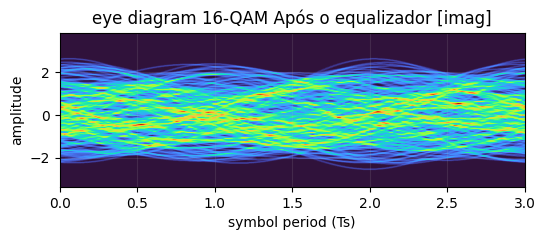
\includegraphics{figuras/nb4_out_17.png}
\end{frame}

\begin{frame}
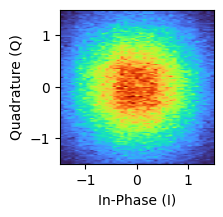
\includegraphics{figuras/nb4_out_18.png}
\end{frame}

\begin{frame}
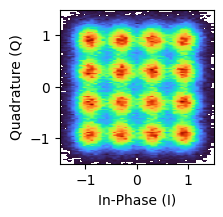
\includegraphics{figuras/nb4_out_19.png}
\end{frame}

\begin{frame}
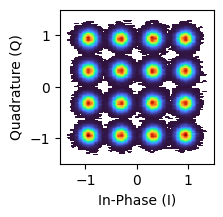
\includegraphics{figuras/nb4_out_20.png}
\end{frame}

\begin{block}{Desempenho BER vs SNR com e sem equalizador}
\phantomsection\label{desempenho-ber-vs-snr-com-e-sem-equalizador}
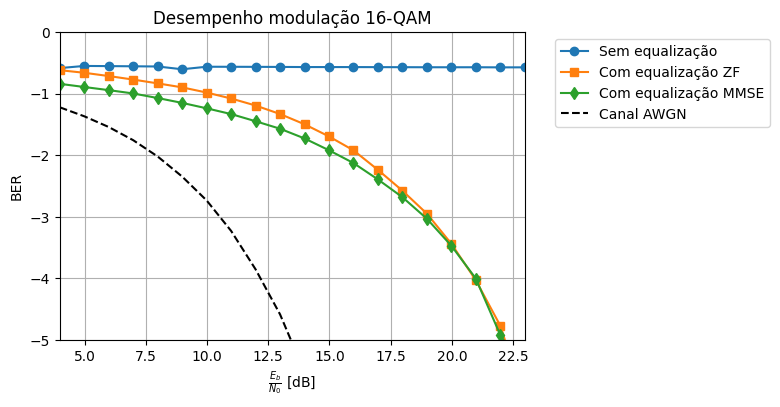
\includegraphics{figuras/nb4_out_21.png}
\end{block}
\end{frame}

\end{document}
